\part Ubica en la recta num\'erica las fracciones $\dfrac{8}{4}$, $\dfrac{9}{4}$, $\dfrac{3}{4}$ y $\dfrac{7}{3}$, escribiendo en el espacio la fracci\'on correspondiente.
\begin{center}
  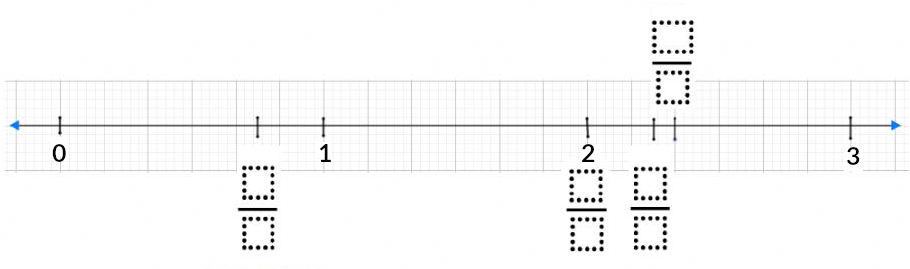
\includegraphics[width=0.8\textwidth]{Images/q1a.png}
\end{center}

\begin{minipage}[c]{\linewidth}
\begin{solutionbox}{9cm}
  Si convertimos las fracciones a n\'umeros decimales podemos compararlos en la recta num\'erica con mayor facilidad:\\
  $\dfrac{8}{4}=2$,\qquad $\dfrac{9}{4}=2.25$, \qquad $\dfrac{3}{4}=0.75$ y \qquad $\dfrac{7}{3}=2.\overline{3}$. \\
    Significa entonces que la fracci\'on que es menor que 1 (que está antes del 1 en la recta num\'erica) es $\frac{3}{4}=0.75$. 
    Despu\'es, la fracci\'on que deberá escribirse debajo del n\'umero 2 es $\frac{8}{4}=2$. La siguiente fracci\'on con un valor
     mayor a 2 es $\frac{9}{4}=2.25$; y la \'ultima que corresponde al n\'umero con el valor m\'as grande es $\frac{7}{3}=2.\overline{3}$,
     que deber\'a colocarse en la \'ultima posici\'on. \\
  \begin{center}
    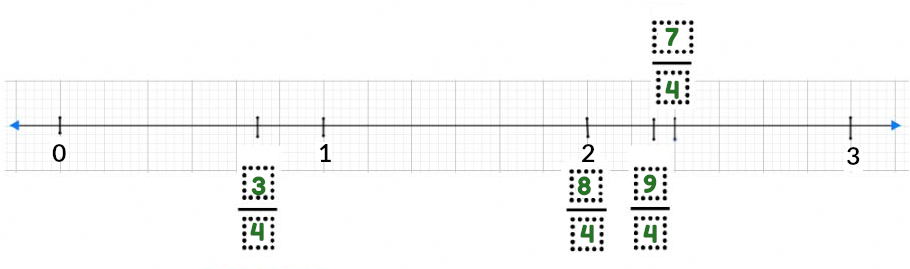
\includegraphics[width=0.8\linewidth]{Images/q1d.png}
  \end{center}
  
\end{solutionbox}
\end{minipage}
